\chapter{Evacuation Planning: An Integrated Approach}
\label{ch:evacuation}
% ##################################################################################################################

\hfill \textbf{Author:} Gregor Lämmel, Christoph Dobler, Hubert Klüpfel 

\begin{center} 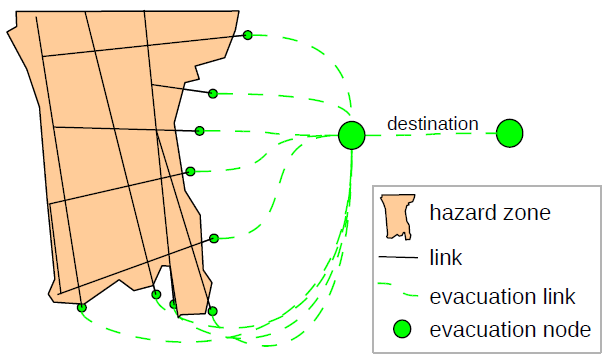
\includegraphics[width=0.4\textwidth, angle=0]{extending/figures/Evacuation/evacuation} \end{center}

\editdone{This text has undergone the professional edit. Please no grammatical changes anymore! They are most-probably wrong.}

\createStandardInformation{evacuation}{\lstinline|RunEvacuationExample| class}{evacuation}{\citet{Laemmel_PhDThesis_2011, 00LaemmelKluepfelNagel2009EvacPadangAtBookTimmermanns}}

% ##################################################################################################################
This chapter presents an integrated approach for performing evacuation simulations with \gls{matsim} using the \gls{grips} contribution. %GRIPS stands for GIS-based Risk-Analysis-, Information-, and Planning-System for Regional Evacuation. 
The approach comprises all workflow steps for performing an evacuation analysis: \ie selecting the evacuation area and defining the population, specifying  behavioral parameters (\ie  pre-movement time distribution and mode of evacuation---car or pedestrian) and analyzing the simulation output. These steps can all be performed within one graphical user interface. Additionally, two extensions of \gls{matsim} for simulating public transport and changing the network during simulation (\ie network change events) are accessible from the \gls{gui}. In this chapter, the steps for performing such an integrated analysis are described and illustrated based on the Hamburg-Wilhelmsburg example. A detailed case study based on this scenario is described in Chapter~\ref{ch:hhw}, as well as in \citet{00DurstAtAl2012PEDGRIPSAppl,Hugenbusch2012Bachelor}.

% ##################################################################################################################
\section{Related Work}
Simulation of evacuation processes has attracted much attention in recent decades; reasons include increases in frequency and severity of natural hazards jeopardizing various populations and regions, as well as (social) disasters~\citep{Rodr2006HBoDisasterResearch}. Another factor is the availability of large-scale, fast simulation models and tools. \citet{Laemmel_PhDThesis_2011} discusses such a model employed as a contribution to \gls{matsim}. Basically, this model implements the same iterative learning approach as that applied to ``regular'' transport scenarios. In the first instance, the cost function comprises only travel times, albeit a combination of travel time and travel distance; a cost function has been investigated as well~\citep{00LaemmelKluepfelNagel2009EvacPadangAtBookTimmermanns}. 
Artificial agents represent evacuees trying to improve their evacuation plans from iteration to iteration, by creating new evacuation plans more responsive to the evolving situation. 
A typical simulation run comprises 500-1\,000\,iterations. 
%If, after any iteration, the best-response dynamic produces the same evacuation plans as those just performed, the system has reached a steady state. This steady state would be a pure strategy Nash equilibrium for the cost function. There is, however, no guarantee that the system ever converges to a steady state. Thus,~\citet{Laemmel_PhDThesis_2011} refers to a Nash equilibrium approach.
%\ah{explained elsewhere}
The model is applied to a tsunami-related evacuation of Padang city in Indonesia \citep[e.g.,][]{00TaubenboeckEtAl2012ConcludingLastMilePaperNatHazards,00GosebergEtAl2012LastLastMile}; some scenario details are discussed in Chapter~\ref{ch:padang}. 

Additional evacuation simulation-related work in \gls{matsim} is presented by \citet{Dobler_PhDThesis_2013}. The main difference to this chapter's approach is that agents are allowed to adapt their plans spontaneously, using \gls{matsim}'s within-day replanning framework \citep{DoblerEtAl_TRR_2012} (Chapter~\ref{ch:withinday}). 
Based on a behavioral model, agents coordinate their actions on a household level. If a household is, \eg not complete when the evacuation starts, each member estimates time needed to return home, as well as the time required to leave the actual evacuation area. Then, the household decides whether meeting at home and leaving together is preferable to each member leaving on its own.
Since the behavioral model is implemented on an agent, respectively household level, individual attributes such as children present in the household, or availability of a car, can be taken into account.
In contrast to regular \gls{matsim} simulations, only a single iteration is performed. Since the agents can optimize their plans continuously using real time information, no further replanning is necessary. As a result, agents do not foresee future events like traffic jams caused by people leaving the threatened area.

An independent evacuation scenario, not using \gls{grips}, is presented in Chapter~\ref{ch:aliaga}.

The remainder of this chapter is organized as follows: Section~\ref{grips:install} gives a brief description on how to set up and run \gls{grips}. 
A short start guide for \gls{grips} is presented in Section~\ref{evac:section:fifteenminute}. Obtaining the required input data is discussed in Section~\ref{grips:input}. Detailed instructions on how to use \gls{grips}'s \lstinline|ScenarioManager|, running simulations and analysis is given in Section~\ref{grips:scm}. This chapter concludes with a brief outlook in Section~\ref{grips:outlook}.

% ##################################################################################################################
\section{Download MATSim and GRIPS}
\label{grips:install}
Although the \gls{matsim} version \lstinline|0.6.0-SNAPSHOT| is referred to here, the package should also work with later versions of \gls{matsim}.
\begin{enumerate}\styleEnumerate
\item 
Download the current nightly build of \gls{matsim} and \gls{grips} from
\url{http://matsim.org/files/builds/}
\item 
Unzip the \lstinline|Matsim_rxxxxx.zip|, \lstinline|Matsim_libs.zip| and\\
 \lstinline|grips-0.6.0-SNAPSHOT-rxxxxx.zip|.
\item 
Move the \lstinline|grips-0.6.0-SNAPSHOT-rxxxxx.jar| and \lstinline|libs| folder from the \lstinline|grips-0.6.0-SNAPSHOT-rxxxxx| directory one level up, 
\ie to the directory, where \lstinline|MATSim_rxxxxx.jar| is located.
\end{enumerate}

Test configuration by invoking\\ 
\begin{lstlisting}
java -cp grips-0.6.0-SNAPSHOT.jar;MATSim_rxxxxx.jar
   org.matsim.contrib.grips.scenariomanager.ScenarioManager
\end{lstlisting}
(It is advisable to copy that command to a file \lstinline|grips.bat|---or \lstinline|grips.sh|, if using a Unix-like operation system. One can then run that file instead of typing the command.)

% ##################################################################################################################
\section{The Fifteen-Minute Tour}
\label{evac:section:fifteenminute}
For just a quick impression, the following steps can be performed within a few minutes:
\begin{description}\styleDescription
\item[OSM] Go to \url{www.openstreetmap.org}, search for the desired place and download a (small) \gls{osm} file. Please choose a small area, \eg 100\,meters by 100\,meters; this is sufficient to begin and size of the exported area is limited. For larger areas, a direct download from sites like \url{www.geofabrik.de} is preferable (see next section).
\item[Run] the \lstinline|ScenarioManager| as described in the previous section.
\item[Create] a scenario by clicking the leftmost button first and then \lstinline|New|. Go to the directory where the designated project should be saved and name the project file (\eg \lstinline|london.xml| or \lstinline|scenario.xml|).
\item[Specify] the path of the \gls{osm} file (by clicking \lstinline|Set| next to network) and the output directory. Leave area and population file as it is, \gls{grips} will handle this.
\textbf{This step must be performed only once. After the scenario-file has been saved, one can open it in the \lstinline|ScenarioManager|.}
\item[Sample size] Set the sample size to 0.1, using the mouse or the cursor buttons on your keyboard.
\item[Departure] Specify the departure time distribution. Plausible values are: normal distribution, $\mu$ and $\sigma$ 600\,seconds (10\,minutes), earliest 300\,seconds, latest 1200\,seconds (20\,minutes).
\item[Save] the scenario file.
\item[Area] Switch to the area tab. One can define the circular evacuation area by keeping the left mouse button pressed and defining the center and radius. Do not forget to save changes.
\item[Population] Switch to the population tab and define the population (handling is similar to area). Do not forget to save changes.
\item[Convert] Switch to the next tab and convert the scenario to \gls{matsim} input files by clicking the \lstinline|run| button. The \gls{matsim} files will be stored in the output directory specified in the beginning.
\item[Run] the \gls{matsim} simulation by skipping the next two tabs/buttons (road closures and buses) and switching to the simulation tab (with the 
% little \ah{little ``M'' or ``m''?}
 ``M'' for \gls{matsim} on the computer screen). Click \lstinline|run|. This will take a while.
\textbf{If an output directory (\eg from a previous run) already exists, it will be renamed.}
\item[Analyze] your simulation results by switching to the final tab after the simulation is finished.

\end{description}

% ##################################################################################################################
\section{Input Data (any Place and any Size)}
\label{grips:input}
The only external input necessary for performing an evacuation analysis with \lstinline|org.matsim.contrib.grips| is an \gls{osm} file.
One can download \gls{osm}.
In this tutorial, we will use the file for Hamburg, Germany. Please go to \url{http://download.geofabrik.de/europe/germany/hamburg.html} and download the \lstinline|hamburg-latest.osm.bz2| file. This is the only initial preparation needed. Everything else can be done with the \lstinline|ScenarioManager| of the \gls{gui}.

% ##################################################################################################################
\section{Scenario Manager}
\label{grips:scm}
The scenario setup, evacuation simulation, and analysis are handled by the \lstinline|ScenarioManager| from the \gls{matsim} contribution package \lstinline|org.matsim.contrib.grips|, 
% =====================================================================================================
\subsection{Scenario Configuration}
At startup, the \lstinline|ScenarioManager| offers the option to either: define a new scenario configuration or open an existing one from a \gls{xml} file, which then can be modified. Figure~\ref{chap:evac:fig:sc_man} shows a screenshot of a scenario configuration in the \lstinline|ScenarioManager| and the corresponding \gls{xml} file, respectively.

\createfigure%
{Illustration of a configuration}%
{Illustration of a configuration opened in the \lstinline|ScenarioManager| and as \protect\gls{xml} file}%
{\label{chap:evac:fig:sc_man}}%
{%
  \createsubfigure%
  {\lstinline|ScenarioManager|}%
{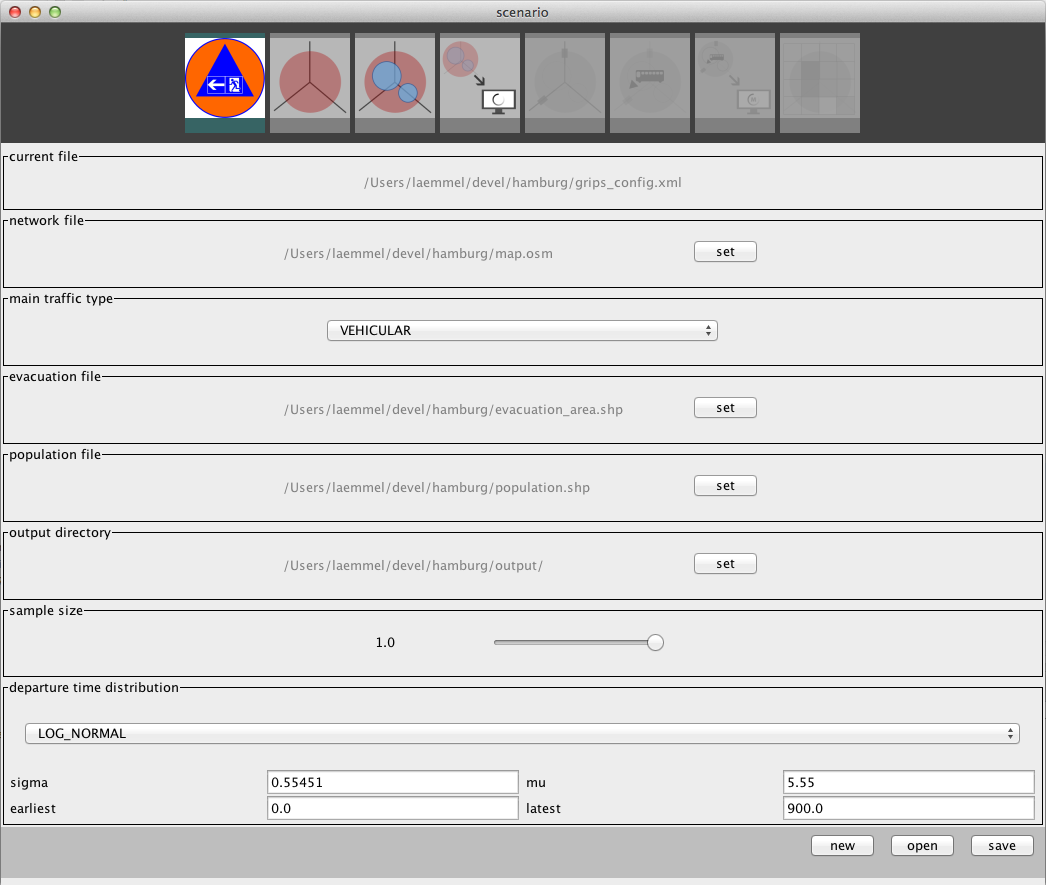
\includegraphics[width=.475\linewidth]{extending/figures/Evacuation/grips_config}}
  {}%
  {}%
  \createsubfigure%
  {XML file}%
{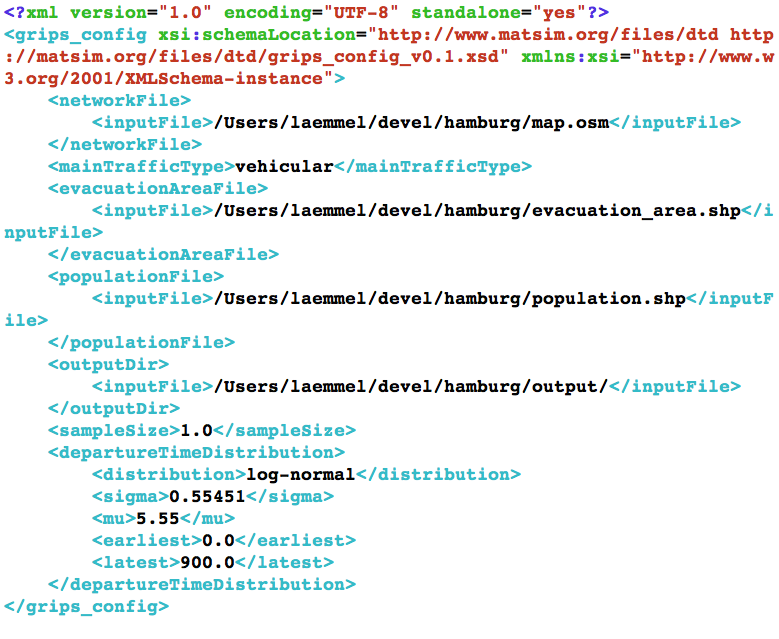
\includegraphics[width=.475\linewidth]{extending/figures/Evacuation/grips_config_xml}}
  {}%
  {}% 
}%
  {}%

The evacuation scenario is specified by the following parameters:
\begin{itemize}\styleItemize
\item The path to the network file covering the evacuation area: currently, \gls{osm} \gls{xml} files are supported (\lstinline|*.osm|).
\item The main traffic type for the simulation:this can either be: \lstinline|VEHICULAR| or \lstinline|PEDESTRIAN|. Depending on the choice, a vehicular specific (the \gls{matsim} default) or a pedestrian-specific (as discussed in~\citet{00LaemmelKluepfelNagel2009EvacPadangAtBookTimmermanns,Laemmel_PhDThesis_2011}) simulation network will be generated by setting free speed, number of lanes and link  flow capacity in the network.
\item The path to a \gls{esri} shape file describing the extent of the evacuation area, depicted by a simple polygon. This file does not have to be in place right from the beginning; it can be produced manually by the \lstinline|ScenarioManager| itself, as discussed later.
\item The path to an \gls{esri} shape file detailing the size and distribution of the affected population. This file comprises a set of simple polygons; each polygon has an additional attribute for the number of persons residing at a location inside that polygon. The evacuation area file can be produced with help of the \lstinline|ScenarioManager|.
\item The path to the output directory where the simulation output and \gls{matsim} scenario files will be stored.
\item The sample size for the \gls{matsim} simulation. A smaller sample size increases the simulation performance, while a larger size might increase accuracy of the results. Typical values are 1.0, 0.1, or 0.01, depending on the scenario and available computing resources.
\item Departure time distribution defines the distribution from which departure times for the simulation will be drawn, based on the premise that, in real evacuation situations, all participants probably do not start evacuation simultaneously. 
People tend to perform pre-evacuation activities before they start, including: picking up relatives, packing food, clothes, valuable belongings, etc. 
Since number and duration of these activities differsby individual, population departure times are unknown quantities. The \lstinline|ScenarioManager| supports three different distributions: (Dirac-delta, normal, and log-normal). If the user chooses the Dirac-delta distribution, then all evacuees will start simultaneously, which might be the worst case~\citep{00LaemmelKluepfel2012InfluenceOfDepartureTimeDistribution}. By choosing the normal distribution, departure times for individuals are drawn from a normal distribution with mean $\mu$ and standard deviation $\sigma$, where the parameters $\mu$ and $\sigma$ are given in seconds. As an example, setting $\mu = 1800$ and $\sigma =  900$ will result in a departure time distribution where, on average, after 30\,minutes 50\,\% of the population has departed and 68.3\,\% of the population departs in time intervals of 30\,minutes $\pm$ 15\,minutes. If the user chooses log-normal as the distribution, departure times are drawn from a log-normal distribution, where $\mu$ and $\sigma$ are the parameters of the associated normal distribution (a discussion on this matter is given below). The parameters \emph{earliest} and \emph{latest} determine the earliest and latest possible departure time. The normal and log-normal departure time distribution are truncated accordingly.
\end{itemize}
%
The departure time distribution is perhaps the most tenuous parameter to set; the authors found no holistic research into this matter. 
In general, it seems reasonable to assume that many people start evacuating at the same time, or soon after the evacuation order has been issued and as time proceeds, fewer and fewer people are left to depart. 
This requires a departure time distribution that has a probability density function beginning with a steep positive gradient, leveling out slowly after a peak. The probability density function of a log-normal distribution produces this kind of curve; log-normal and normal distributions are closely related. If the random variable $Y$ is normal distributed, then $X = \text{exp}(Y)$ is log-normal distributed. The expected value $E[X]$ and the variance $Var[X]$ are
\begin{equation}
E[X] = \text{exp}(\mu + \frac{\sigma^2}{2})
\end{equation}
and 
\begin{equation}
Var[X]=\text{exp}(2(\mu+\sigma^2))-\text{exp}(2\mu+\sigma^2).
\end{equation}
Conversely, if the expected value and variance is given, $\mu$ and $\sigma$ of the associated normal distribution can be obtained as follows:
\begin{equation}
\sigma = \sqrt{\text{log}(1+\frac{Var[X]}{(E[X])^2})}\label{chap:evac:eq:sigma}
\end{equation}
and 
\begin{equation}
\mu = \text{log}(E[X] - \frac{1}{2}\sigma^2).\label{chap:evac:eq:mu}
\end{equation}
If users wish to generate a population with departure times following a log-normal distribution, it is hard to see how $\sigma$ and $\mu$ will determine the outcome. It is much more convenient to consider expected value and variance. Given Equation~(\ref{chap:evac:eq:sigma}) and Equation~(\ref{chap:evac:eq:mu}), a conversion from expected value and variance to $\sigma$ and $\mu$ is straightforward.

% =====================================================================================================
\subsection{Evacuation Area}% and population}
The \lstinline|ScenarioManager| integrates modules for the evacuation area definition and distribution of the affected population. The so-called evacuation area selection module allows the user to define the evacuation area by drawing either a simple polygon or circle on a map. The application can make use of either a WMS-provider or a tile map provider (\eg \gls{osm}) as background map renderer. Zooming and panning is restricted to the bounding box of the \gls{osm} network file provided in the scenario configuration. An illustration of the evacuation area selector is given in Figure~\ref{chap:evac:fig:area_pop}. In addition to defining a new evacuation area, a pre-existing one can also be loaded into the \lstinline|ScenarioManager|. The requirements for a pre-existing evacuation area file are:
\begin{itemize}\styleItemize
\item It has to be provided as a \gls{esri} shape file.
\item The evacuation area must be defined as a simple polygon or a multi-polygon containing one, and only one, simple polygon.
\item The coordinate reference system for polygon in the \gls{esri} shape file must be set correctly. 
\end{itemize}
Due to the high likelihood of error, this approach is recommended for experienced users only.

Later in the process, the \lstinline|ScenarioManager| takes the evacuation area to cut out an evacuation network. However, after cutting out the evacuation net, there is no particular node as a target for the route calculation, as evacuees have more than one safe place as a destination. Instead, in the underlying domain, every node outside the evacuation area is a possible destination for an evacuee seeking an escape route. Thus, the evacuation problem is, in general, a multi-destination problem. To resolve this, the ; all exit links (\ie links that originate inside the evacuation area and terminate outside the evacuation area) are connected, using virtual links with infinite flow capacity and zero length, to a super-node; all evacuation routes are routed to the super-node. This way, the problem is reduced to a multi-source single-destination problem. And thus, finding the shortest path from any node inside the evacuation area to this super-node and, in consequence, to safety, can efficiently be solved. For technical reasons, a super-link is added to the super-node and the evacuees are routed to that link (see the image at the beginning of this chapter).

% =====================================================================================================
\subsection{Evacuation Demand}
The process of defining the population distribution is similar to that of the evacuation area, differing because population is distributed over circles drawn on the map. The user can draw an arbitrary number of those circles and define population figures individually for each circle. Figure~\ref{chap:evac:fig:area_pop} illustrates the population editor. 
%
\createfigure%
{The evacuation area and the population distribution can be defined with an integrated \protect\gls{gis} application}%
{The evacuation area and the population distribution can be defined with an integrated \protect\gls{gis} application}%
{\label{chap:evac:fig:area_pop}}%
{%
  \createsubfigure%
  {Evacuation area}%
{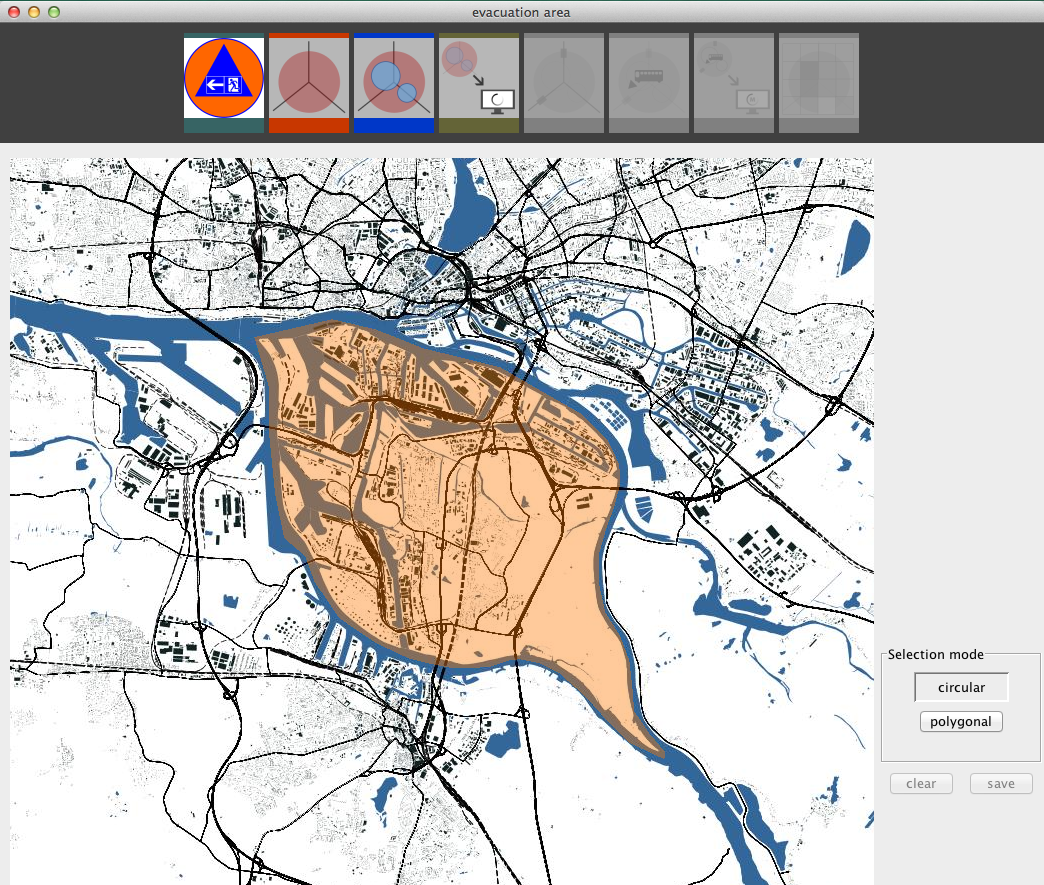
\includegraphics[width=.475\linewidth]{extending/figures/Evacuation/evac_area_sel}}
  {}%
  {}%
  \createsubfigure%
  {Population distribution}%
{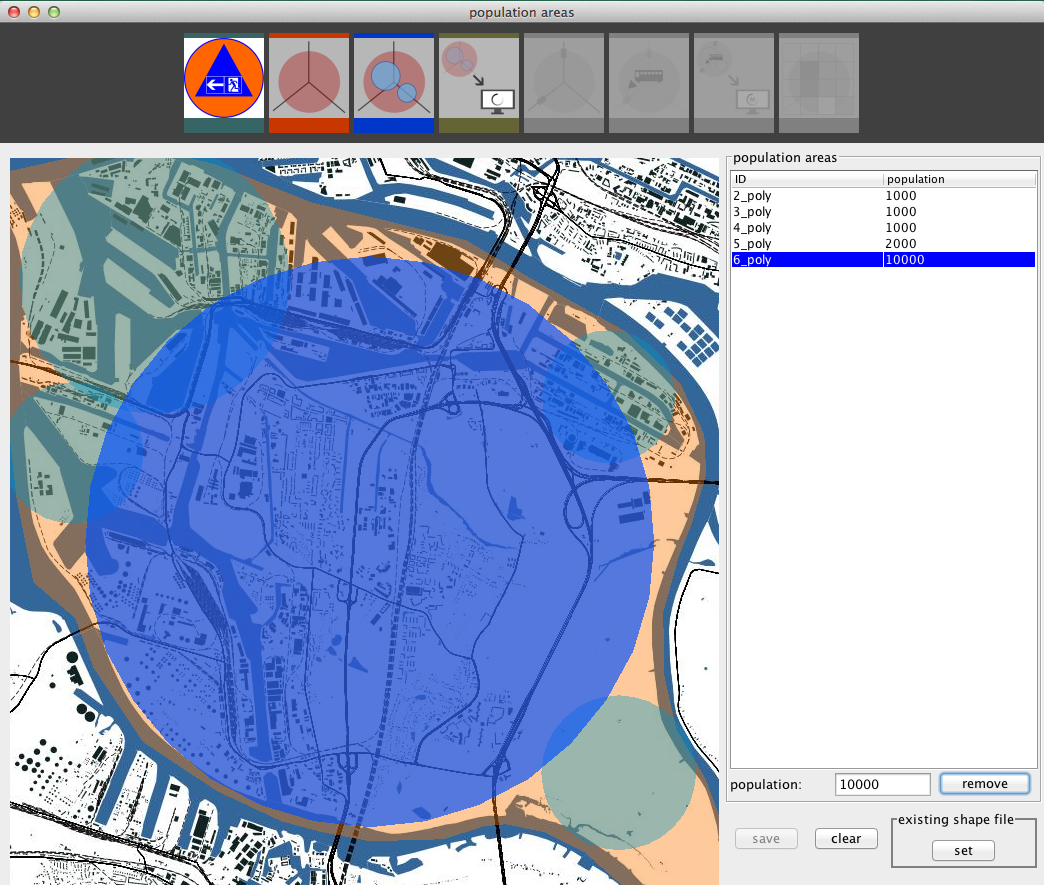
\includegraphics[width=.475\linewidth]{extending/figures/Evacuation/pop_sel}}
  {}%
  {}% 
}%
  {}%
%
The population editor offers only basic functionality to define a population distribution. For every circular area, the \lstinline|ScenarioManager| produces as many agents as required and assigns each agent a random coordinate inside the circular area. However, in \gls{matsim} agents depart on links, so the \lstinline|ScenarioManager| calls the \lstinline|getNearestLink()| method defined in \lstinline|NetworkImpl|. Thus, agents will depart on links inside and possibly near the circular areas. 

In the current version, it is impossible to use a predefined demand for the simulation. Extending the simulation package in this way would be straightforward, but is out of this work's scope.

% =====================================================================================================
\subsection{Road Closures}
In real situations, all exiting roads are often not available for the evacuation, because:
\begin{itemize}\styleItemize
\item They might be impassable due to the event (often the case in flooding-related evacuations).
\item The authorities might want to keep roads open only for action/help traffic.
\item In some situations, like hurricane evacuations, lane direction on motorways might be reversed to increase flow capacity in one direction.
\item The authorities have detailed evacuation plans in place, with pre-planned evacuation routes; road closures might be necessary to force evacuees onto certain routes.
\end{itemize}
The actual planning of road closures can be a complex undertaking; not all attributes can be integrated into a simple tool for rapid evacuation planning. Nevertheless, the \lstinline|ScenarioManager| offers a tool to create time-dependent road closures. An illustration of the road closures editor is given in Figure~\ref{fig:evac_editor}(b).

\createfigure%
{Road closures can be edited by an integrated \protect\gls{gis} application.}%
{Road closures can be edited by an integrated \protect\gls{gis} application. For every link, the direction and closure time can be defined. Tool that lets the user define bus stop locations and schedules}%
{\label{fig:evac_editor}}%
{%
  \createsubfigure%
  {Road closures}%
{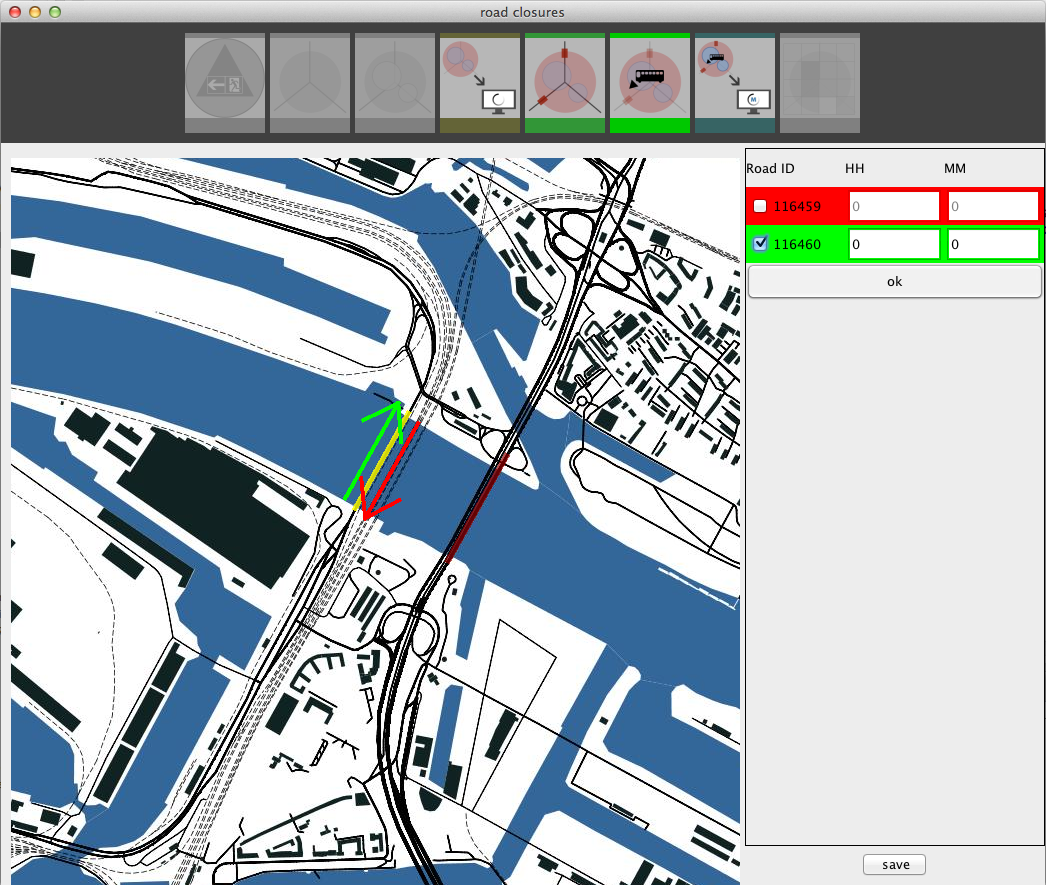
\includegraphics[width=.475\linewidth]{extending/figures/Evacuation/rd_closure_detail}}
  {}%
  {}%
  \createsubfigure%
  {Bus stop locations and schedules}%
{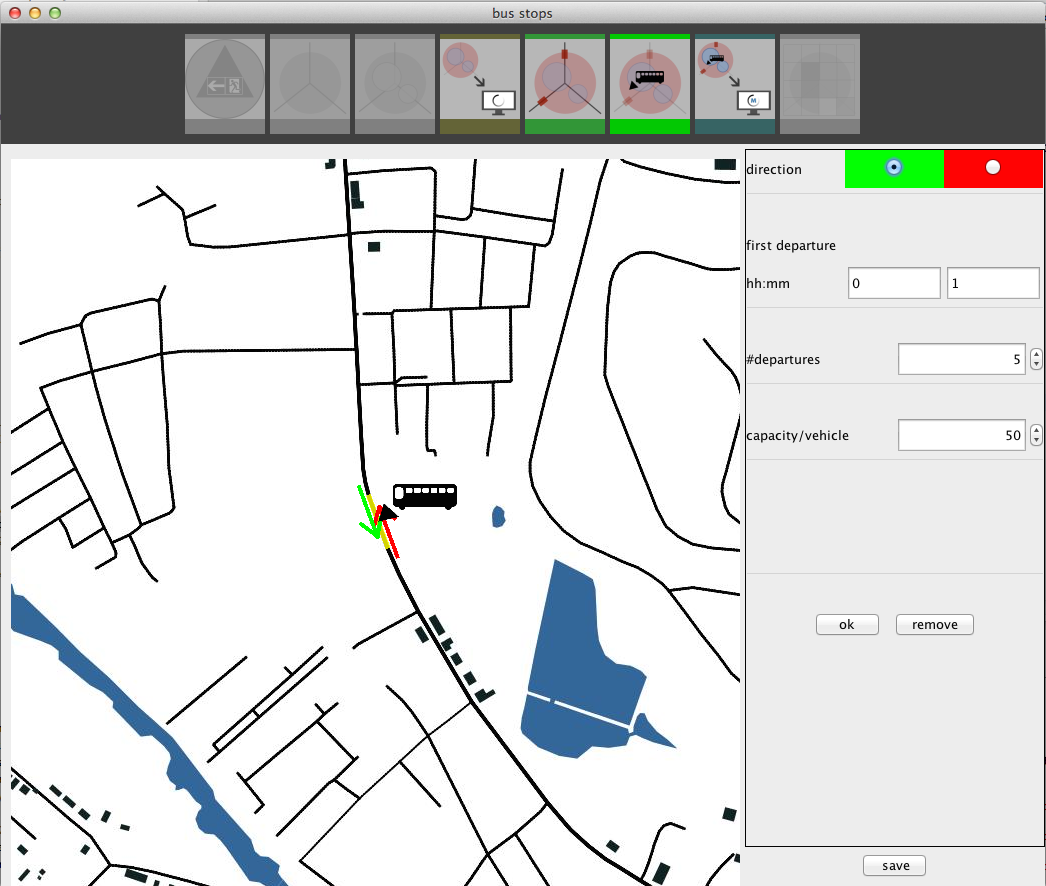
\includegraphics[width=.475\linewidth]{extending/figures/Evacuation/bus_stops}}
  {}%
  {}% 
}%
  {}%

Road closures are stored as \lstinline|NetworkChangeEvents| and handled as time-dependent network attributes in \gls{matsim}~\citep{LaemmelGretherNagel2009TimeDependentNetworks}.

% =====================================================================================================
\subsection{Bus Stop Editor}
Usually, not everyone has access to a private car. In the event of an evacuation, those people often rely on public transport. In regions prone to natural disasters, local authorities normally have detailed evacuation plans in place, probably including evacuation by public transport. Consequently, it is important to have a tool available to help  integrate public transport into to the simulation framework. The \lstinline|ScenarioManger| offers this possibility by defining bus stops and bus schedules in the interactive \gls{gui}. Figure~\ref{fig:evac_editor}(b) gives an example of the bus stop editor. In addition to location, the user can define when the first bus will serve a bus stop, how many buses overall will serve this particular bus stop and these buses' capacity. 
The \lstinline|ScenarioManager| transforms the inputs made into the \gls{gui} into a \gls{matsim} compatible transport schedule, enriching the scenario while using the same simulation model. Details about public transport simulations with \gls{matsim} are given in Chapter~\ref{ch:pt}. A tutorial can be found on the \gls{matsim} webpage \url{http://matsim.org/docs/tutorials/transit}.

Limitations of the public transport evacuation approach in this project are:
\begin{itemize}\styleItemize
\item Each bus serves one and only one bus stop, perhaps a realistic assumption.
\item Buses always take the shortest path from their designated bus stops to the safe area. As the shortest path is not necessarily the fastest, this approach might lead to avoidable delays. Some newer research investigates optimization of bus lines with respect to traffic demand and traffic conditions~\citep{Neumann2014PhD}. Implementing such optimization techniques in the evacuation context is a topic of future research.
\end{itemize}

% =====================================================================================================
\subsection{Running the Scenario}
The \lstinline|ScenarioManager| runs the evacuation simulation in a way similar to other transport simulation studies with \gls{matsim}. 
At the beginning, an evacuation plan is assigned to each evacuee. 
An evacuation plan describes how the evacuee intends to reach the safe area.
If the evacuee leaves by car or on foot, the plan is essentially comprised of a route (typically the shortest) from home to the safe area. For evacuees who are depart by public transportation, the plan can be much more complex. All these evacuation plans will be executed in the mobility simulation; after this terminates, all plans are scored by travel time. 
The shorter a plan's travel time is, the higher is the score it receives. After this step, evacuees' plans are revised; some will receive new plans, while others continue with the current ones. This step is called re-planning. Mobility simulation, scoring, and re-planning are repeated in a loop for a predefined number of iterations; evacuees' individual performance improves over the iterations. 
In general transport studies, this approach emulates real-world travelers' behavior when they perform their daily commutes and try to find better travel alternatives. Evacuations, however, are singular events where such day-to-day re-planning would not occur. We argue here that the chosen iterative learning approach could be seen as the evacuees' anticipation of the conditions expected during an evacuation. 
People familiar with their surroundings would probably avoid roads that obviously constitute bottlenecks during an evacuation. Nevertheless, far more research is needed to definitively answer how people choose evacuation routes, or how many learning iterations are required to realistically reflect assumed anticipation skills adequately. As a rule of thumb, running 100\,learning iterations re usually sufficient to achieve results constituting a lower evacuation times boundary.   

% =====================================================================================================
\subsection{Analysis}
After the last iteration has finished, the \lstinline|ScenrioManager| enables the analysis module. The analysis model evaluates the performed simulation run, using a number of different methods. 
\begin{itemize}\styleItemize
\item The cumulative arrival curve tells the user the number of persons evacuated over time. From this curve, the user can, for example, learn at what time 50\,\% of the population has reached a safe destination.
\item The \gls{gis}-based evacuation time analysis draws a grid over the evacuation area and computes, for every grid cell, average evacuation time. The evacuation times are indicated by different colors; the analysis modules run a quantiles-based clustering analysis for each cell. The size of cells can be varied  by the user.
\item The \gls{gis}-based clearance time analysis is performed in the same way as the evacuation time  analysis. The clearance time of a cell is the time when the last evacuee leaves that cell. This evacuee is not necessarily the one who also started his/her evacuation inside the corresponding cell, but might also be one who crosses that cell at some when during the evacuation.
\item A similar quantiles-based clustering approach is used for the link utilization analysis. The link utilization analysis results help the user to identify most-used roads during the evacuation.
\end{itemize}
The analyses can be run for every single iteration for which the \gls{matsim} \lstinline|Controler| has dumped an events file (every 10th iteration by default). An overview of the analysis module is given in Figure~\ref{chap:evac:fig:analysis}

\createfigure%
{Screenshot of the analysis module showing \protect\gls{gis}-based evacuation time analysis and the evacuation curve}%
{Screenshot of the analysis module showing \protect\gls{gis}-based evacuation time analysis and the evacuation curve}%
{\label{chap:evac:fig:analysis}}%
{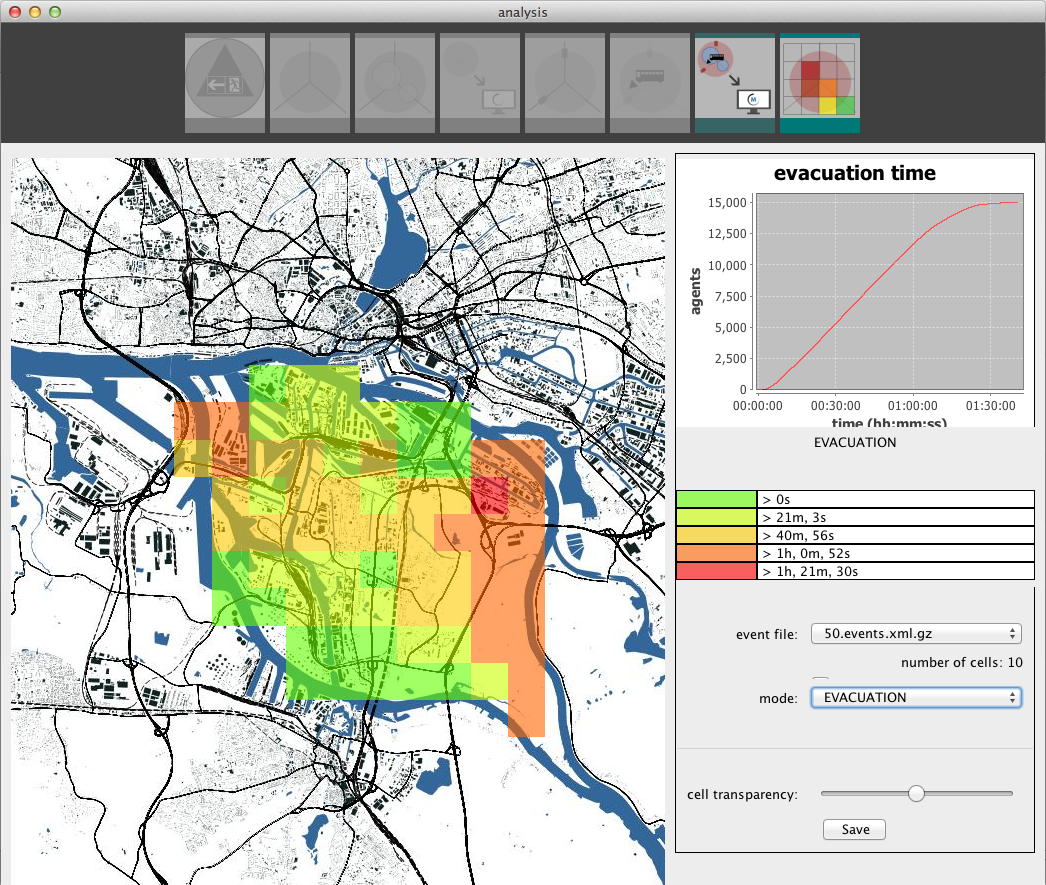
\includegraphics[width=1\textwidth]{extending/figures/Evacuation/it50_evac_time}}
{}

% ##################################################################################################################
\section{Conclusion}
\label{grips:outlook}
This chapter demonstrates how rapid evacuation planning can be performed with help of the \gls{grips} contribution. The \gls{grips} contribution provides an interactive \gls{gui} to perform this task.
The only required external input is a network file extracted from \gls{osm}, thus a simple scenario can be setup, simulated, and analyzed in less than an hour. Obviously, for an in-depth evacuation analysis of a certain area, much expert knowledge is needed that a simple \gls{gui} can not supply. Still, for a rapid appraisal and for demonstration purposes, \gls{grips} offers a powerful and easy-to-use tool. In the future, we plan to integrate a more advanced public transport planning tool based on~\citet{Neumann2014PhD}. Work is also ongoing to develop a more sophisticated pedestrian simulation model based on the theoretical framework given in~\citet{00FloetteroedLaemmel2014BiPedFnd}.

% ##################################################################################################################
